\documentclass[a4paper,12pt,reqno]{amsart}
\usepackage[T1]{fontenc}
\usepackage[utf8]{inputenc}
\usepackage{amsmath, amsthm, amssymb,amscd, mathrsfs, amsfonts, mathtools}
\usepackage{xcolor}
\usepackage{tikz}
\usetikzlibrary{hobby,knots,graphs,graphs.standard,arrows.meta}
\usetikzlibrary{decorations.pathreplacing}

\begin{document}

        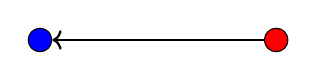
\begin{tikzpicture}

% Vertices
\node[draw, circle, fill=red, minimum size=2pt, inner sep=3pt, text=white] (Red) at (3,0) {};
\node[draw, circle, fill=blue, minimum size=2pt, inner sep=3pt, text=white] (Blue) at (0,0) {};

% Directed edge from Red to Blue
\draw[->, thick] (Red) -- (Blue);

\end{tikzpicture}

\end{document}